\documentclass{standalone}

\usepackage{tikz}
\usetikzlibrary{shadows}
\usetikzlibrary{positioning}
\usetikzlibrary{arrows}
\usetikzlibrary{shapes.misc}
\definecolor{dkgreen}{rgb}{0,0.6,0}
\begin{document}

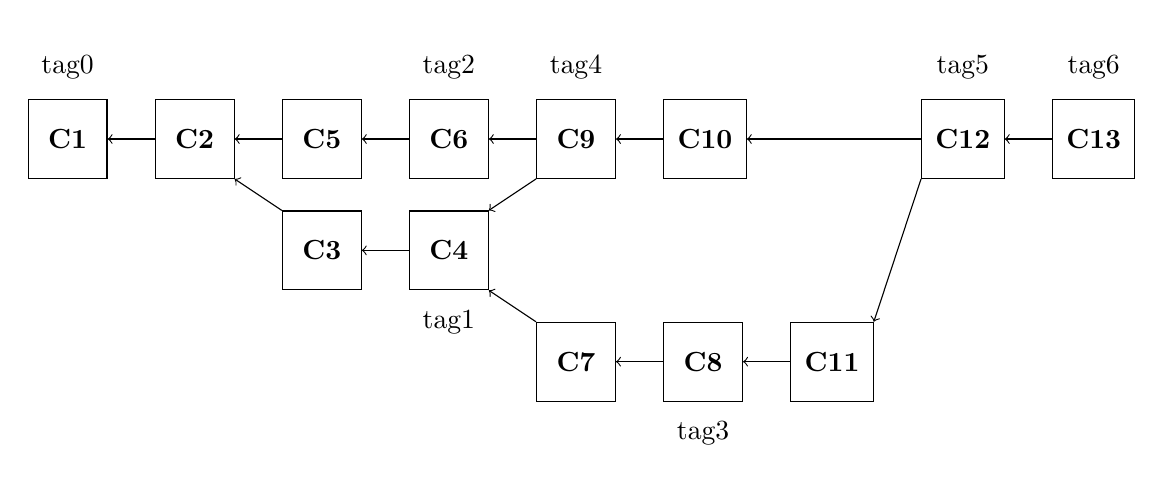
\begin{tikzpicture}[node distance=4mm and 6mm, common/.style={draw, fill=white, inner sep=5pt, font=\bfseries},minimum size=10mm]
\tikzstyle{fakenode}=[]
\tikzstyle{texto}=[]

\node (C1) [common] at (0, 0) {C1};
\node (C2) [common, right=of C1]   {C2};
\node (C3) [common, below right=of C2]  {C3};
\node (C4) [common, right=of C3]  {C4};
\node (C5) [common, right=of C2]  {C5};
\node (C6) [common, right=of C5]  {C6};
\node (C7) [common, below right=of C4]  {C7};
\node (C8) [common, right=of C7]  {C8};
\node (C9) [common, right=of C6]  {C9};
\node (C10) [common, right=of C9]  {C10};
\node (C11) [common, right=of C8]  {C11};
\node (fakenode) [fakenode,right=of C10]  {};
\node (C12) [common, right=of fakenode]  {C12};
\node (C13) [common, right=of C12]  {C13};

% arriba
\draw [<-](node cs:name=C1, anchor=east) -- (node cs:name=C2, anchor=west);
\draw [<-](node cs:name=C2) -- (node cs:name=C5);
\draw [<-](node cs:name=C5) -- (node cs:name=C6);
\draw [<-](node cs:name=C6) -- (node cs:name=C9);
\draw [<-](node cs:name=C9) -- (node cs:name=C10);
\draw [<-](node cs:name=C10) -- (node cs:name=C12);
\draw [<-](node cs:name=C12) -- (node cs:name=C13);

% medio
\draw [<-](node cs:name=C2, anchor=south east) -- (node cs:name=C3, anchor=north west);
\draw [<-](node cs:name=C3, anchor=east) -- (node cs:name=C4, anchor=west);
\draw [<-](node cs:name=C4, anchor=north east) -- (node cs:name=C9, anchor=south west);

% abajo
\draw [<-](node cs:name=C4, anchor=south east) -- (node cs:name=C7, anchor=north west);
\draw [<-](node cs:name=C7) -- (node cs:name=C8);
\draw [<-](node cs:name=C8) -- (node cs:name=C11);
\draw [<-](node cs:name=C11, anchor=north east) -- (node cs:name=C12, anchor=south west);

% tags
\node [texto,above=of C1,yshift=-5mm] {tag0};
\node [texto,below=of C4,yshift=5mm] {tag1};
\node [texto,above=of C6,yshift=-5mm] {tag2};
\node [texto,below=of C8,yshift=5mm] {tag3};
\node [texto,above=of C9,yshift=-5mm] {tag4};
\node [texto,above=of C12,yshift=-5mm] {tag5};
\node [texto,above=of C13,yshift=-5mm] {tag6};
\end{tikzpicture}


\end{document}